\section*{Empirical evidence for nonnegative sparse coding in the brain}

\subsection*{Reconstructing stimulus spaces using sparse, parts-based representations}

An influential paper by Lee and Seung \cite{LeeSeung1999}
found that applying \ac{NMF} to a database of face images
yielded sparse, localized features that resembled parts of a face
\revise{(Fig.~\ref{fig:NMF|reconstruction}A)}.
In their case, \ac{NMF} acted on a
$F \times S$ data matrix \textbf{V},
whose rows corresponded to distinct features of the input 
(e.g., $F$ different pixels of an image)
and whose columns corresponded to different stimuli or 
observations of those features
(e.g., $S$ different images).
\ac{NMF} was used to decompose the matrix into two reduced-rank matrices
(Fig.~\ref{fig:NMF|reconstruction}, \revise{inset})
whose linear combination could be weighted such that the product of \textbf{W} and \textbf{H} provided an accurate reconstruction of \textbf{V}.

On its surface, \ac{NMF} would appear to be unrelated to 
the mechanisms underlying 
artificial or biological neural networks;
however, it was Lee and Seung's intuitive mapping of these variables onto
a neural network that forms the cornerstone 
of our conception of the \ac{NSC} framework:
In the context of \ac{NSC}, \textbf{V} and \textbf{H} correspond to activation values of two distinct neuronal populations, which are connected to each other via synaptic weight values in \textbf{W}.
A particular image, in this case encoded by $F = 19 \times 19 = 361$ 
pixels $v_1, \ldots, v_F$
(i.e., a column of \textbf{V}),
could be reconstructed by a linear mixing of a total of $B$ encoding variables
$h_1, \ldots, h_B$ (i.e., a column of \textbf{H}).
A single encoding variable $b \in 1, \ldots, B$ 
influences multiple image pixels,
owing to the fan-out of the connections from the encoding variable.
As a result, a particular image of a face 
(Fig.~\ref{fig:NMF|reconstruction}\revise{A})
could be accurately represented by a linear combination of 
a small number ($B = 49$) of encoding variables or `basis images'.
Such a representation is reminiscent to neural processing in \ac{IT},
an area in the ventral visual `what' stream
involved in encoding high-level object identity
\cite{BrincatConnor2004,Majaj2015},
where images of whole faces can be linearly reconstructed
using responses of approximately $200$ neurons
that each respond to a certain set of physical facial features
\cite{ChangTsao2017}.

\begin{figure}[!h]
	\centering
	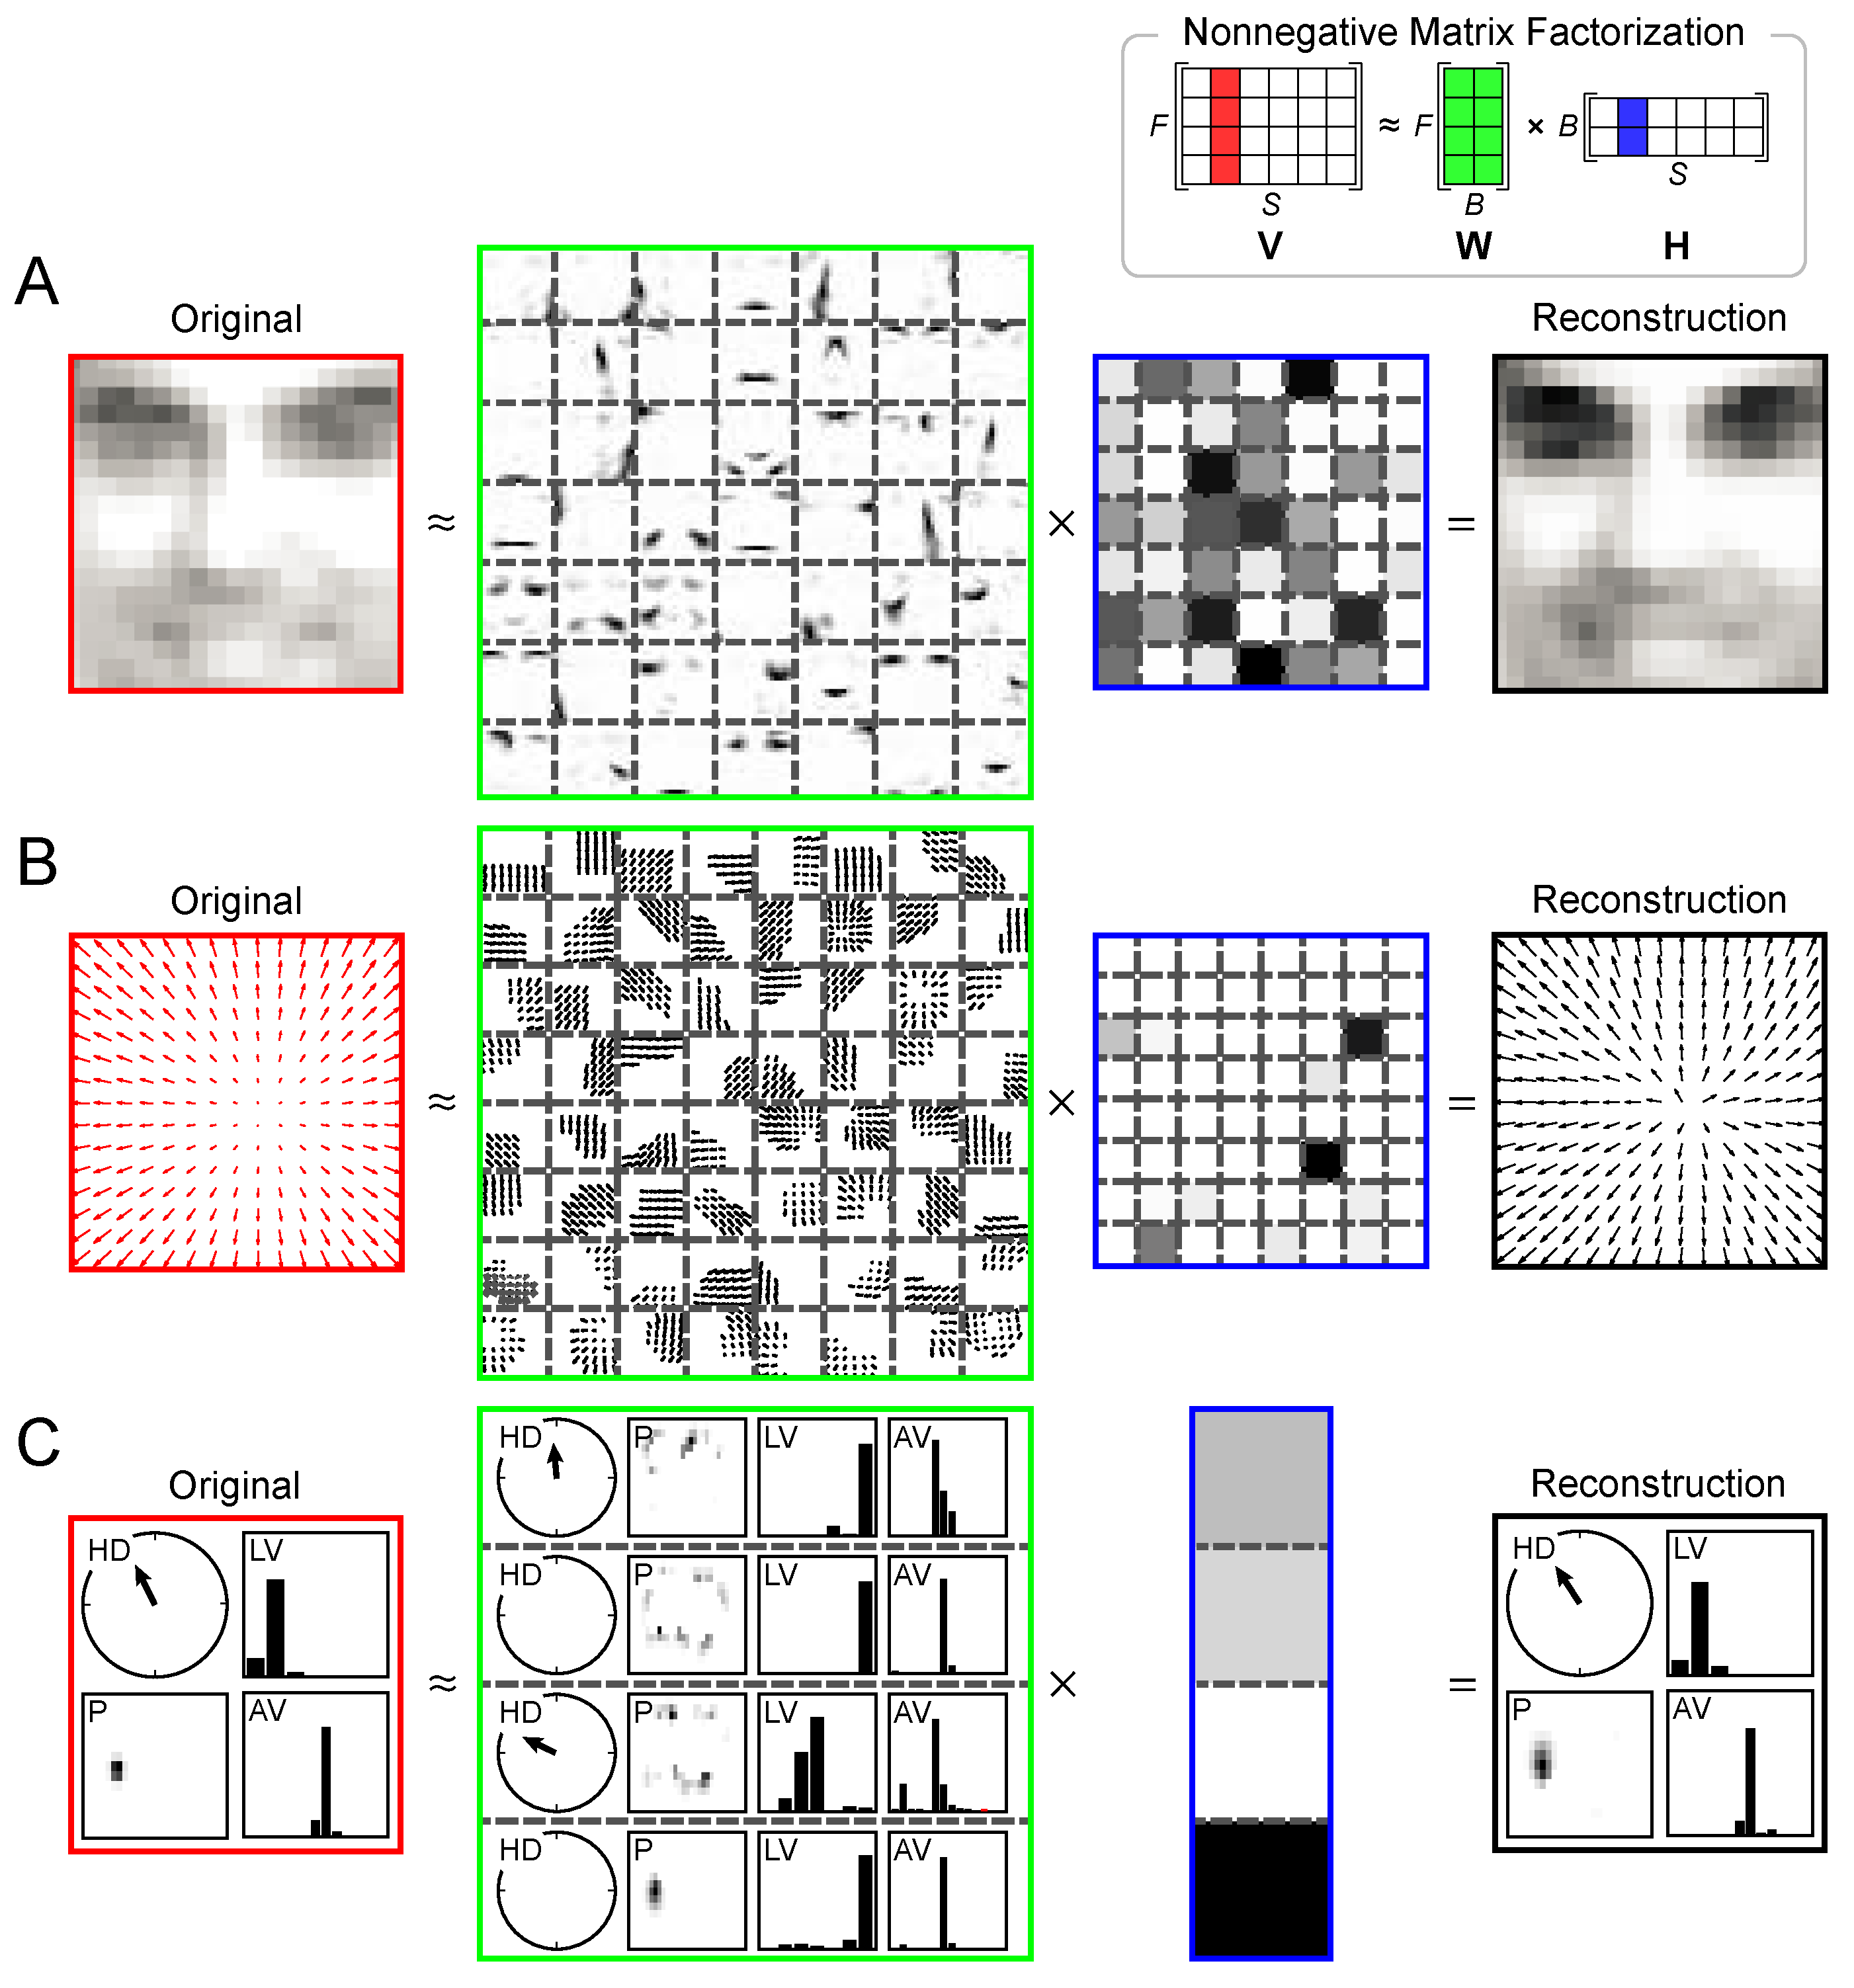
\includegraphics[width=\textwidth]{fig-rev1-reconstruction}
    \caption{\revise{Sparse and parts-based representations recovered by \ac{NMF}
             resemble receptive fields across brain regions.
             \Ac{NMF} (inset) can reconstruct a} data matrix \textbf{V}
             ($F$ features x $S$ stimuli)
             from two reduced-rank matrices \textbf{W}
             (containing $B$ basis vectors) and \textbf{H}
             (containing the hidden coefficients of the decomposition).
             Any individual input stimulus (i.e., column in \textbf{V}, \revise{red})
             can be reconstructed from a linear combination
             \revise{(i.e., column in \textbf{H}, blue)}
             of a set of basis vectors (i.e., all columns in \textbf{W}, 
             \revise{green}).
             A) A facial image can be reconstructed from a sparse activation
                of simulated \acs{IT} neurons that
                preferentially respond to parts of faces
                (adapted from \cite{LeeSeung1999}).
             B) An optic flow field can be reconstructed from a sparse
                activation of model \acs{MSTd} neurons that prefer various
                directions of 3D self-translation and self-rotation
                (adapted from \cite{Beyeler2016}).
             C) A rat's 2D allocentric position and route-based direction of
                motion can be reconstructed from a sparse activation of
                model \acs{RSC} neurons that prefer an intricate combination of
                linear velocity (LV), angular velocity (AV), head direction (HD)
                and 2D position (P).
                For the sake of clarity, only the 4 most contributing hidden
                coefficients (out of 30) are shown.}
	\label{fig:NMF|reconstruction}
\end{figure}


Remarkably, such a parts-based representation is not specific to
information processing in \ac{IT};
the same principle can be extended to other areas of the visual system,
such as the \ac{MSTd},
which is part of the visual motion pathway \cite{Beyeler2016}.
Neurons in \ac{MSTd} respond to relatively large and complex patterns
of retinal motion (`optic flow'),
owing to input from direction and speed selective neurons in the \ac{MT}
(for a recent review, see \cite{Orban2007}).
Although \ac{MSTd} had long been suspected to be involved in the
analysis of self-motion,
the complexity of neuronal response properties has made it difficult
to experimentally investigate how neurons in \ac{MSTd}
might perform this function.
However, when \revise{our group} 
applied \ac{NMF} to 
\revise{simulated neural activity patterns whose statistical properties
resembled that of experimentally recorded \ac{MT} neurons} 
\cite{Beyeler2016},
\revise{we} found a sparse, parts-based representation of retinal flow
(Fig.~\ref{fig:NMF|reconstruction}\revise{B})
similar to the parts-based representation of faces
encountered by Lee and Seung \cite{LeeSeung1999}.
The resulting `basis flow fields' showed a remarkable resemblance to receptive fields
of \ac{MSTd} neurons, as they \revise{responded}
an intricate mixture of
3D translational and rotational flow components
in a subset of the visual field.
As a result, any flow field possibly to be encountered 
during self-movement through a 3D environment
could be represented by only $B = 64$ simulated \ac{MSTd} neurons,
as compared to $F = 9,000$ simulated \ac{MT} input neurons.
This led to an sparse \revise{and parts-based} population code,
where any given stimulus could be represented
by only a small number of simulated \ac{MSTd} neurons (population sparsity)
\cite{Beyeler2016}.

Analogously, \ac{NSC} can explain response properties
of neurons outside the visual system, 
such as in the \acf{RSC}, an area important for navigation and spatial memory \cite{Miller2014,Nelson2015,VannAggleton2009}.
Neurons in the \ac{RSC} conjunctively encode multiple variables related to the environment and one's position and movement within it
\revise{(e.g., position, head direction, linear velocity, and angular velocity)},
allowing the representation of spatial features of the environment 
with respect to multiple reference frames \cite{AlexanderNitz2015}.
\revise{When our group applied \ac{NMF} to neurophysiological data from
\ac{RSC} neurons while rats ran back and forth on a W-shaped track
(for experimental details, see Supplementary Materials),
we again found a sparse and parts-based representation for behaviorally
relevant variables such as the animal's position, head direction, 
and movement direction (Fig.~\ref{fig:NMF|reconstruction}C).
Interestingly, model \ac{RSC} neurons encoded these variables with respect
to multiple frames of reference (e.g., head direction: allocentric,
linear velocity: route-based).
\mikeNote{Are these reference frames stated correctly?}
Once again, the dimensionality of the stimulus space was drastically reduced
from $F = 417$ input neurons to a set of $B = 30$ model \ac{RSC} neurons.}

Although there seems to be a consensus that 
information-theoretic explanations are relevant 
when investigating the early visual system,
higher-order brain areas are often considered to be specialized for
performing tasks
(e.g., recognizing objects, making decisions, navigating an environment),
rather than the efficient encoding of information.
However, the finding that \ac{NSC} could be used to explain neuronal responses
in the visual and retrosplenial cortices introduces the possibility that it might
apply elsewhere in the brain.
This introduces the possibility that \ac{NSC} might in fact
be a general principle to which neuronal computations adhere.

In fact, sparse (and potentially parts-based) representations have been observed
in olfactory, auditory, \revise{somatosensory, parietal,} and motor cortices
(see Table~\ref{table:listEvidence}).
\revise{In the following subsections, we will look at some examples, and explain
why some of these refs are in the table. We will discuss how population codes
differ in different brain areas, and what that means for sparse and parts-based.}
\mikeNote{words}


\begin{table}[!ht]
\begin{adjustwidth}{-2.25in}{0in}
	\centering
	\caption{Nonnegative sparse coding in the brain.
    We list a group of brain regions for which there is experimental evidence of certain features associated with NSC (`X': evidence exists, `?': has yet to be investigated).
   For each brain region, the left-hand side of the table lists experimental evidence for sparse and/or parts-based representations, whereas the right-hand side lists computational support that NSC can describe receptive fields or response properties within that region.}
%     \scriptsize
	\begin{tabular}{r|rrr|rr}
	 &  &  \textbf{Parts-} & \textbf{Experimental} & \textbf{Modeled} & \textbf{Computational} \\
	\textbf{Area} & \textbf{Sparse} & \textbf{based} & \textbf{evidence} & \textbf{by NSC} & \textbf{ support} \\ \hline
    Retina & X & X & \cite{Onken2016,Liu2017} & X & \cite{Onken2016,Liu2017} \\
    Early visual cortex & X & X & \pbox{5cm}{\cite{OlshausenField1996,HoyerHyvarinen2002,Hoyer2003,vanHateren1998}} & X & \pbox{5cm}{\cite{OlshausenField1996,Hoyer2003,Carlson2013,Hyvarinen2001}} \\
    Ventral visual stream & X & X & \pbox{5cm}{\cite{Wachsmuth1994,FreiwaldTsao2010,ChangTsao2017}} & X & \pbox{5cm}{\cite{LeeSeung1999,Hosoda2009}}  \\
    Dorsal visual stream & X & X & \pbox{5cm}{\cite{BenHamed2003,PougetSejnowski1997,PougetSnyder2000}} & X & \cite{Beyeler2016} \\
    Auditory cortex & X & ? & \cite{Hromadka2008} & ? & ? \\
 	\revise{Somatosensory} cortex & X  & ? & \cite{Kerr2007} & ? & ?  \\
 	Olfactory cortex & X & ? & \cite{Koulakov2011} & ? & \cite{MorenoBoteDrugowitsch2015}  \\
    \revise{WHAT ABOUT PARIETAL} & & &  &  &   \\
    \revise{WHAT ABOUT FRONTAL} & & &  &  &   \\
    Retrosplenial cortex & X & X & \cite{AlexanderNitz2015} & X & present paper \\
    Motor cortex & X & ? & \pbox{5cm}{\cite{GrazianoAflalo2007,Turner2000}} & ? & \cite{Vargas2010decoding} \\
    Basal ganglia & X & ? & \cite{BarGad2000, BarGad2003_Review}  & X & \pbox{5cm}{\cite{BarGad2003_Review}, advanced RDDR} \\
    Hippocampus & X & ? & \cite{Poli2017} & ? & ? \\
	\end{tabular}
    \label{table:listEvidence}
\end{adjustwidth}
\end{table}



